\documentclass[12pt]{article}

\usepackage{amsmath}
\usepackage{amssymb,amsfonts}
\usepackage{graphicx}
\usepackage{hyperref}
\usepackage{longtable}

\pagestyle{plain}

\hypersetup{
	colorlinks=true,
	urlcolor=blue
}

\setlength{\textwidth}{5.7truein}
\setlength{\textheight}{8.7truein}
\setlength{\oddsidemargin}{3.0mm}
\setlength{\evensidemargin}{3.0mm}
\setlength{\topmargin}{-12.5truemm}
\setlength{\parindent}{0.0truemm}
\parskip=2mm

\title{\bf Sprint Zero Return Brief}
\author{THEM - Typed HTML5 Evaluation Machine \\ Carl Hattenfels \\ Scott Heiner \\ Shen Yong Lau \\ Robert Meyer \\ Brendan Miller \\ David Uebergang}

%\date{}
%% See what happens if the above line has a % symbol at the start, so that it's ignored!

%%%%%%%%%%%%%%%%%%%%%%%%%%%%%%%%%%
\begin{document}

\maketitle

\section*{Return Brief}

Our team plans to implement a web based application that allows users to evaluate HTML5 files and entire website structures. This brief was provided by Lorna MacDonald, the course co-ordinator of the University of Queensland (UQ) course ``Introduction to Web Design" (DECO1400). Specifically, this application will be utilised by the students of that course, providing them with an application to check the validity of their files. This external factor, however, will have little bearing on our final product, as Lorna has allowed us freedom in how we choose to implement her specification. This application aims to provide an easy way for students to check their code quickly and efficiently, and the web application allows for this to be conducted independent of the user's platform. However, the use of this application is broad, and could be utilised by anyone needing verification of HTML files and websites to high standards.

The application will analyse the HTML content of individual pages and determine how closely the file's style conforms to ``best practice'' criteria. The common issues this program will check for are:
\begin{itemize}
\item Structural / syntactical
\begin{itemize}
\item Multiple instances of singular tags - html, head, body, footer
\item Incorrect page structure (html, head, body, footer - where tags are missing or in the wrong order)
\item Form elements not being contained in a form object
\item Failure to close tags that require a closing tag
\item Incorrect nesting of tags - resulting in overlapping html tags
\item Incorrect table structures - cells not in rows, different numbers of cells in rows where colspans are not specified
\item Missing title tag in head
\item Missing required attributes (src for img, href or name for a, href for link etc)
\item Use of short tags - self-closing tags not having forward slash
\item Use of PHP in a html file (that is, not using php extension)
\item Form elements
\begin{itemize}
\item incorrect or misspelt type attributes for inputs
\item missing value attributes,
\item radio inputs with the same id,
\item inputs missing name attribute - causes issues when accessing via \\ JavaScript or PHP
\end{itemize}\end{itemize}
\item Deprecated elements:
\begin{itemize}
\item Use of frames
\item Use of deprecated presentational tags (b, i, small etc)
\end{itemize}
\item Accessibility:
\begin{itemize}
\item Form elements not having labels
\item Missing alt tags on images - accessibility standards not followed
\end{itemize}
\item Poor practice/Miscellaneous:
\begin{itemize}
\item Using tables for layout
\item Semantic issues - multiple H1's, incorrect use of headings
\item Multiple elements with the same value for the id attribute - causes issues when they begin to work with JavaScript and the DOM.
\item Special characters used or non-ASCII character used.
\end{itemize}\end{itemize}

Users can also upload zipped files of entire websites that the application checks for correct files linkage. The application will be able to recognise: 
\begin{itemize}
\item Incorrect linking to local files - images, CSS, JavaScript and other HTML files. This could be due to files being in a different location to the link specified or due a mismatch in the case used in the filepath. In this case, the application will look into the files provided and give a possible correction.
\item  Presence of an index.html file. This is something that students regularly forget which causes issues when they publish to a web server.
\item  Cleanliness of file structure - placement of CSS files into a CSS directory, of image files into an images directory etc.
\end{itemize}

The application will utilise XHTML, CSS, PHP, as well as Python for parsing the files. The Python program locates the errors of the uploaded files and returns a JSON object (through JSON-RPC) which the website parses and displays to the user. Javascript will be utilised to provide more detail - when the user clicks on an error, it will expand to reveal more information about that error. For the duration of development, it will be hosted on a personal server, but after development may be placed on a UQ web server. These constraints make it feasible for us to develop this application, based on the team's knowledge in these languages.

Two scenarios where this application will be utilised are validation of individual files and validation of websites. In the first case, a typical user of the application navigates to the website before clicking either ``Direct Input" or ``Upload File". On the Direct Input page, the user can copy in a single page of HTML for the program to verify, while on the Upload File page, the user can select multiple HTML files to be uploaded and validated. For validation of websites, the user navigates to the website and then selects ``Upload ZIP", after which they may upload a zip file of their website for analysis.

To show our team is capable of implementing this solution, we have created an early prototype of the web application. This prototype can be viewed at \underline{\url{http://underwaterfall.com}}. 

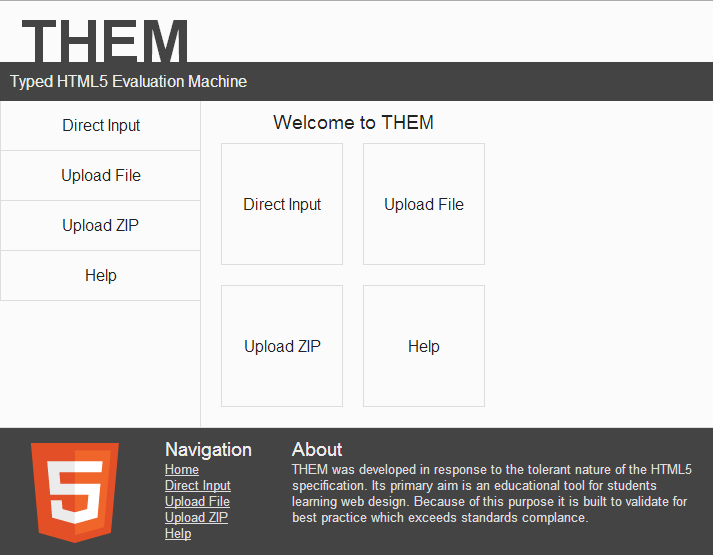
\includegraphics[scale=0.65]{index.png}

We have connected the website to a Python program via JSON-RPC, such that when a user types some text into the form provided on the ``Direct Input" page, they are sent to a page which returns what they wrote, along with how many lines they sent (provided by the Python program). This can obviously be extended to any parsing of the text using Python, which is the focus of the application.

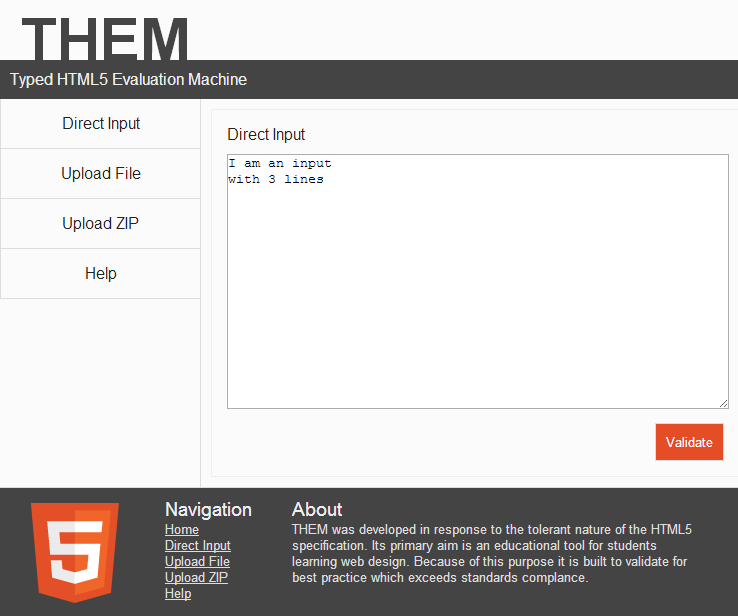
\includegraphics[scale=0.65]{direct_input.png} \\ \\

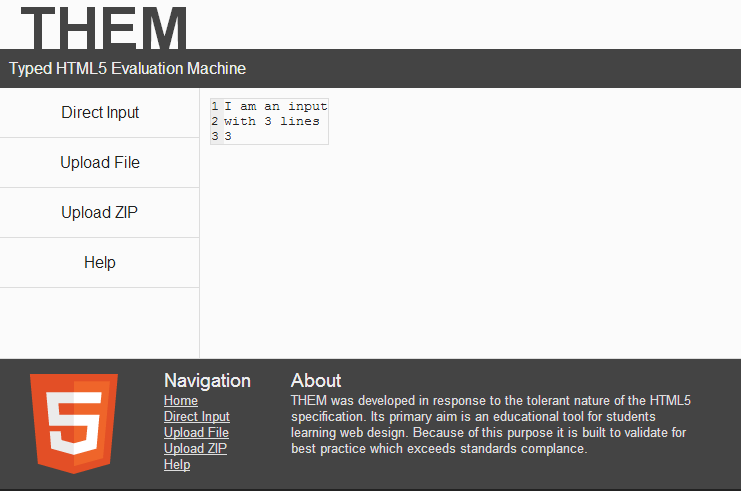
\includegraphics[scale=0.65]{returned_input.png}

Also, uploading a file or a zip will currently return information about that file or zip, but in the future will display information about the errors in the files.

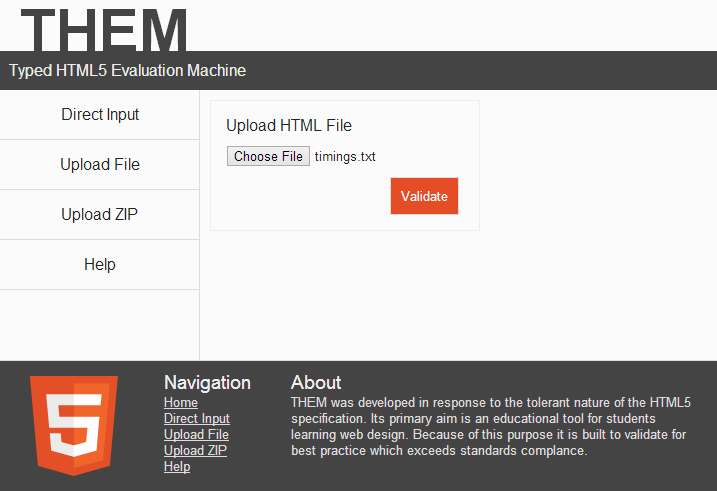
\includegraphics[scale=0.65]{upload_file.png} \\ \\

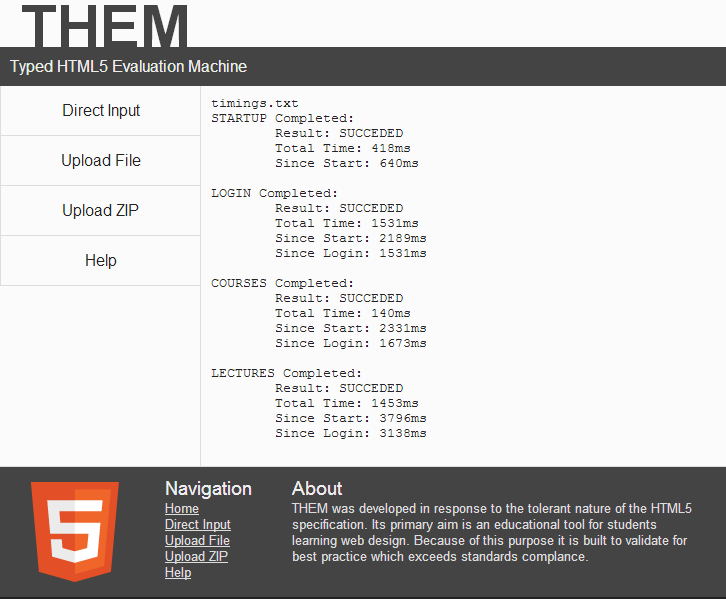
\includegraphics[scale=0.65]{upload_file_return.png} \\ \\

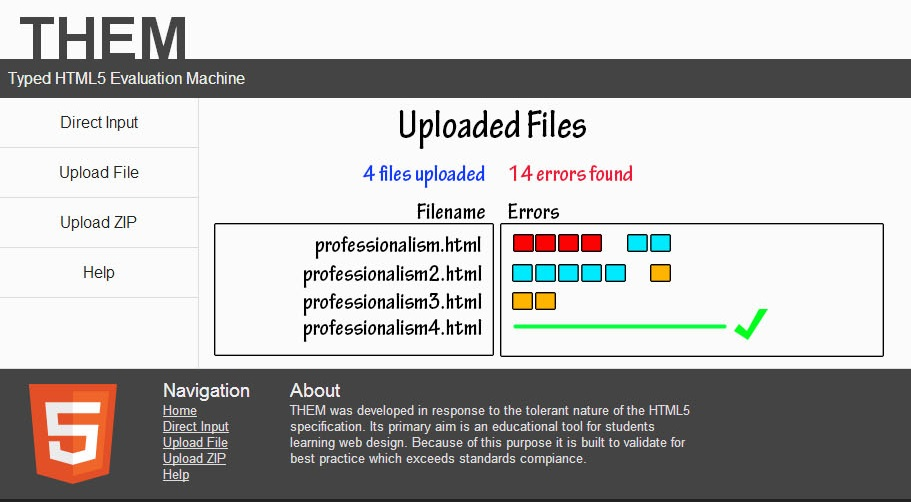
\includegraphics[scale=0.65]{uploadedfiles.jpg}

The above is an initial digital prototype of the planned ``Uploaded Files" page. It shows a clear view of the number of errors and types of errors, and allows users to click on the name of files to delve further into the errors contained in their code.

\section*{Quote}

\subsection*{Work Breakdown}

\begin{longtable}{|l|l|}
    \hline
    {\bf TASK}                           & {\bf DOUBLED HOURS} \\
    \hline
    {\bf Initial Upkeep}                 & ~             \\
    Server Set-Up                        & 2             \\
    Library Searching                    & 2             \\
    Python Familiarisation               & 4             \\
    HTML Familiarisation                 & 4             \\
    PHP Familiarisation                  & 4             \\
    Initial Charter Documentation        & 4             \\
    Design Mockups                       & 6             \\
    Profile Scoping                      & 14            \\
    \hline
    ~                                    & 40            \\
    \hline
    ~                                    & ~             \\
    ~                                    & ~             \\
    ~                                    & ~             \\
    ~                                    & ~             \\
    {\bf Implementation}                 & ~             \\
    {\em Front End}                      & ~             \\
    Upload Page                          & ~             \\
    HTML/PHP                             & 2             \\
    Javascript                           & 2             \\
    Direct Input Page                    & ~             \\
    HTML/PHP                             & 2             \\
    Javascript                           & 2             \\
    Single File Upload                   & ~             \\
    HTML/PHP                             & 2             \\
    Javascript                           & 2             \\
    Zip File Upload Page                 & ~             \\
    HTML/PHP                             & 2             \\
    Javascript                           & 2             \\
    Help Page                            & ~             \\
    HTML/PHP                             & 2             \\
    Javascript                           & 2             \\
    Errors/Warnings Overview Page        & ~             \\
    HTML/PHP                             & 6             \\
    Javascript                           & 6             \\
    File Structure Overview Page         & ~             \\
    HTML/PHP                             & 4             \\
    Javascript                           & 4             \\
    CSS (Sitewide)                       & 20            \\
    \hline
    ~                                    & 60            \\
    \hline
    {\em Back End}                       & ~             \\
    Python JSON-RPC Server Functionality & 8             \\
    Python HTML5 Parsing Functions       & ~             \\
    StructuralErrors                     & 20            \\
    Syntactical Errors                   & 60            \\
    Deprecated Elements Errors           & 10            \\
    Accessibility Errors                 & 10            \\
    Poor practice/Miscellaneous Errors   & 20            \\
    Documenting Error Messages           & 10            \\
    File Structure Parsing (Python)      & 40            \\
    Unzip Folder Structure (Python)      & 20            \\
    PHP JSON-RPC Functionality           & 8             \\
    Database Setup                       & 4             \\
    Database Temporary File Storage      & 8             \\
    \hline
    ~                                    & 218           \\
    \hline
    ~                                    & ~             \\
    ~                                    & ~             \\
    ~                                    & ~             \\
    {\bf Testing}                        & ~             \\
    {\em User Testing}                   & ~             \\
    Initial Website Navigation           & 10            \\
    Understanding Errors                 & 20            \\
    Understanding Multiple Files         & 30            \\
    Understanding File Map               & 40            \\
    Help Page Testing                    & 6             \\
    \hline
    ~                                    & 106           \\
    \hline
    {\em Functional Testing}             & ~             \\
    Uploading Files                      & 8             \\
    Error Highlighting and Display       & 24            \\
    Multiple File Uploading and Display  & 16            \\
    Unzipping Files                      & 24            \\
    Display of File Map                  & 40            \\
    General Website Functional Tests     & 20            \\
    \hline
    ~                                    & 132           \\
    \hline
    {\bf Documentation}                  & ~             \\
    Sprint Zero Return Brief             & 12            \\
    Updated Test Plan                    & 12            \\
    User Guide                           & 20            \\
    System Installation Guide            & 10            \\
    Final Report                         & 30            \\
    Marketing Report                     & 6             \\
    \hline
    ~                                    & 90            \\
    \hline
    {\bf Marketing}                      & ~             \\
    Marketing Scoping                    & 10            \\
    Completing Marketing Materials       & 6             \\
    \hline
    ~                                    & 16            \\
    \hline\hline
    {\bf \em Total}                      & 662           \\
    \hline
\end{longtable}

\subsection*{Supplementary Costs and Total Cost}

The only supplementary cost related to this project is server hosting costs, and possible maintenance in the future. In general, this is an ongoing, but inconsequential cost (about \$10/month for hosting, specifically, with variable rates for maintenance decided by the university themselves). We expect UQ to provide this server space. At the costing rate of \$50/hour for a project manager and \$35/hour for everyone else, the total cost of this project comes to \$24,820.

\section*{Risk Analysis}

A project of this nature brings with it some inherent risks. The first and inevitable risk is related to the heavy workload from other subjects during the semester. This workload may influence the work progress of the team members. Consequently, the final product might not meet the client's expectations or even achieve our own benchmark. In order to ease the tension and pressure of every member, the distribution of task allocation and frequency of team meetings has been considered thoroughly. For each job task, there will be at least two people assigned to not only distribute the work but ensure the task can still be completed even when one person is busy. Meetings plays a crucial role here, since this task description and distribution will be discussed at these events. In addition, the project manager will also work as a mediator between members in order to fine-tune the different jobs carried out between the team members such as programming, user interface and documentation.

The difference in our team members' understanding of HTML5 and the understanding of the target audience is another potential risk. It involves the knowledge gap between the creators and those who learn from it. In this case, it is likely that we might create a tool that cannot be understood by the target audience but does meet our client's basic expectations. For instance, the presentation of errors and types of errors the users encounter may be confusing to interpret. Therefore, our project manager has ensured our production timeline involves necessary collaboration with not only our client but also users along the way. This will be covered in more depth in the next paragraph.

Whilst on the topic of our application's compatibility, it is also challenging for our team to deliver a final product that validates HTML5 code completely and efficiently. Since DECO1400 has not yet included HTML5 in its curriculum, we are reliant on previous assignments (which are based on HTML4) to use in our functional testing. In this instance, the worst case scenario would be that the tool issues incorrect errors to end users. In order to mitigate this risk, working closely with our client is necessary. We plan to utilise not only past examples but newer examples provided by our client and examples we personally program. As previously mentioned, our team also plans to conduct user testing in both a laboratory environment and an open area environment. Through consistent user testing of this nature, we can better improve the compatibility of this application with regards to the HTML5 standard.

There is a chance for conflict of ideas, as well as the chance that a large number of concurrent ideas are proposed to solve the same task. This risk most likely can delay our success and progress. Therefore, we have implemented a voting system within our team as well as included policies behind the voting system to ensure these conflicts do not arise. For example, the project manager will have the final decision on the matter if any decision reaches a tied vote. Furthermore, all voting will be most likely be conducted through Facebook, as this is our primary communication method beyond phone messaging and face-to-face meetings.

\newpage
\section*{Supplementary Materials}

As previously mentioned, the prototype can be viewed at \underline{\url{http://underwaterfall.com}}.

\subsection*{Transcripts of Client Meetings}

{\bf Initial Client Meeting}

From: Lorna Macdonald [lorna@itee.uq.edu.au]
Sent: 29 July 2013 17:54
To: Mr Brendan Miller
Subject: Re: HTML Learning Tool - DECO3801
 
Hi Brendan,
That will work fine. See you then.
Cheers,
Lorna

On 29/07/2013, at 4:38 PM, Mr Brendan Miller [brendan.miller@uqconnect.edu.au] wrote:

Ok, how about 11-12 on Thursday?

Thanks,
Brendan

From: Lorna Macdonald [lorna@itee.uq.edu.au]
Sent: 29 July 2013 16:36
To: Mr Brendan Miller
Subject: Re: HTML Learning Tool - DECO3801
 
Hi Brendan,
Unfortunately not - have a meeting then.
Cheers,
Lorna

On 29/07/2013, at 4:23 PM, Mr Brendan Miller [brendan.miller@uqconnect.edu.au] wrote:

Hi Lorna,

Are you free this Wednesday between 9-10 for a meeting with the team?

thanks,
Brendan Miller

From: Lorna MacDonald [lorna@itee.uq.edu.au]
Sent: 29 July 2013 09:51
To: Mr Brendan Miller
Subject: Re: HTML Learning Tool - DECO3801
 
Hi Brendan,
I won't be in today due to unforeseen circumstances. Please accept my apologies. I'm happy to reschedule for later this week.
Cheers,
Lorna 

Lorna Macdonald
Associate Lecturer - School of Information Technology and Electrical Engineering
The University of Queensland
St Lucia, QLD 

Ph. 3365 3335  |  E. lorna@itee.uq.edu.au

On 26/07/2013, at 2:24 PM, ``Mr Brendan Miller" [brendan.miller@uqconnect.edu.au] wrote:

Hi Lorna,

Excellent. We'll see you then.

Thanks,
Brendan Miller

From: Lorna Macdonald [lorna@itee.uq.edu.au]
Sent: 26 July 2013 13:17
To: Mr Brendan Miller
Subject: Re: HTML Learning Tool - DECO3801
 
Hi Brendan,
Certainly, I have a meeting that finishes at 2, so if I'm a little late that's where I'll be. My office ok? 78-325
Cheers,
Lorna

On 26/07/2013, at 12:09 PM, Mr Brendan Miller [brendan.miller@uqconnect.edu.au]
 wrote:

Hey Lorna,

Can we meet with you this coming monday (29th) at 2 for an hour?
I can organise a space if your office doesn't suit, as our team is 6.

thanks,
Brendan

From: Lorna Macdonald [lorna@itee.uq.edu.au]
Sent: 26 July 2013 09:05
To: Mr Brendan Miller
Subject: Re: HTML Learning Tool - DECO3801
 
Hi Brendan,
Glad to hear it. Best times for me are Monday after 2pm, Tuesday after 3, Wednesday before 11 and after 3, Thurs mornings and Friday mornings.
Cheers,
Lorna

On 25/07/2013, at 4:30 PM, Mr Brendan Miller [brendan.miller@uqconnect.edu.au]
 wrote:

Hi Lorna,

I'm writing to you on behalf of my 3801 team. We're going to be building the html
learning tool. We're discussing the design brief amongst ourselves and we'll be in
contact when we want to discuss it in greater detail. Are there certain times of the
week that suit you more than others for consultation?

thanks,
Brendan Miller


{\bf Return Brief}

Wednesday, August 07, 2013 9:27 AM
Lorna Macdonald [lorna@itee.uq.edu.au]
To:
 Mr Scott Heiner 

Hi Scott, 
I'm around until 12. 
Cheers,
Lorna


Wednesday, August 07, 2013 9:15 AM
Mr Scott Heiner [scott.heiner@uqconnect.edu.au]
To:
 Lorna Macdonald

Hi Lorna,

Is there any time today before 1pm when you're free? I wanted to pass the return brief by you before we submit it. Sorry for the late notice on this.

Sincerely,
Scott Heiner

\end{document}